
\documentclass[]{article}
\usepackage[version=3]{mhchem}
\usepackage{natbib}
\usepackage{graphicx}
\usepackage{float}
\usepackage[german]{babel}
\bibliographystyle{abbrvnat}
\usepackage[colorlinks]{hyperref}
\hypersetup{
  citecolor = {blue},
}
\newcommand{\unit}[1]{\ensuremath{\, \mathrm{#1}}}

\title {Einfache und kostengünstige Messung des Methanpotentials mittels der Gasdichte (GD-BMP)\footnote{
  Empfohle Zitierung: 
Hafner, S.D.; Astals, S.; Holliger, C.; Justesen, C.; Koch, K.; Mortensen, J.R.; Weinrich, S. 2021 Gas density-based BMP measurement. Standard BMP Methods document 304, version 2.3., online verfügbar unter: https://www.dbfz.de/en/BMP (abgerufen am TT.MM.JJJJ).
\newline
  Unter \url{https://www.dbfz.de/en/BMP} gibt es eine BibTeX-Datei, die in alle gängigen Litera-
turverwaltungsprogramme importiert werden kann.
}
}
\author{Sasha D. Hafner, Sergi Astals, Christof Holliger, \\ Camilla Justesen, Konrad Koch, Jacob R. Mortensen, \\ S\"oren Weinrich} 

\date{\today \\
\bigskip
\textit{
  Dokument 304.
  Dieses Dokument ist eine deutsche Übersetzung der englischen Originalversion (Version 2.3) von Konrad Koch und S{\"o}ren Weinrich. 
  Dieses Dokument ist Teil der Methodensammlung zur Standardisierung von Batchversuchen (Standard-BMP-Methoden).\footnote{ Weitere Informationen und andere Dokumente unter \url{https://www.dbfz.de/en/BMP}. 
    Alle Dokumentversionen gibt es unter \url{https://github.com/sashahafner/BMP-methods}; dort ist es auch möglich, Änderungen vorzuschlagen.}
}
}

\begin{document}
\maketitle

\section{Einführung}
Das Gasdichte-BMP-Verfahren (GD-BMP) ist eine Methode, die im Gegensatz zu anderen manuellen Verfahren zur Bestimmung des biochemischen Methanpotentials (BMP), keine teuren Gasanalysegeräte erfordert.
Bei dieser Methode werden das Biogasvolumen und der damit verbundene Massenverlust der Flasche  verwendet, um die Biogasdichte zu bestimmen, mit Hilfe derer die Biogaszusammensetzung ermittelt wird.\footnote{Wenn ein Gemisch nur aus zwei Gasen besteht, in diesem Fall \ce{CH4} und \ce{CO2}, kann die Zusammensetzung allein aus der Dichte bestimmt werden.} Anhand des gemessenen Biogasvolumens und des Massenverlustes können die Methanproduktion über die Zeit sowie der vollständige Methanertrag (am Versuchsende) bestimmt werden.
Dieses Dokument enthält ein detailliertes Laborprotokoll für die Anwendung der GD-BMP-Methode.
Die Entwicklung und Validierung der Methode ist in \citet{justesenDevelopmentValidationLowcost2019} beschrieben.
Informationen zu Berechnungen rund um die GD-BMP-Methode gibt es in Dokument 204 auf der Website für Standard-BMP-Methoden \citep{BMPdoc204gasdens}.

\section{Gerätschaften und Zubehör}
\label{sec:equipment}
Für die Anwendung der GD-BMP-Methode sind folgende Gerätschaften und Zubehörteile erforderlich:
\begin{itemize}
    \item Elektronische Waage
    \item Spritzen und Kanülen
    \item Manometer
    \item BMP-Flaschen und Septen
    \item Inkubator
\end{itemize}

Die erforderliche Genauigkeit der Waage hängt von der Menge des erzeugten Biogases ab.
Ganz allgemein gilt, dass die angegebene Genauigkeit\footnote{
  Hersteller geben die Genauigkeit häufig als \glqq Linearität\grqq{} an. Die Genauigkeit entspricht jedoch nicht der Ablesbarkeit, denn dies ist der kleinste Wert, der abgelesen werden kann.} der Skala mindestens 30 mg pro g verwendeter organischer Trockensubstanz (oTS) betragen sollte.\footnote{
  Wenn beispielsweise jeder Flasche 2 g oTS (Substrat) zugegeben werden, muss die vom Hersteller angegebene Genauigkeit mindestens 60 mg betragen (z.B. wären 50 mg ausreichend).}
Wie unten beschrieben, wird die Genauigkeit und Stabilität der Waage als Teil des Protokolls überprüft.

Ein einfaches geschlossenes U-Rohr-Manometer\footnote{
  Ein geschlossenes U-Rohr-Manometer kann aus mit Wasser gefüllten, flexiblen Kunststoffschläuchen und einem einfachen Ventil hergestellt werden. Ein Beispiel dafür ist in Abb. \ref{fig:utube} zu finden.
} oder ein kostengünstiges elektronisches Manometer reicht aus, um zu ermitteln, wann der Druck im Kopfraum nach dem Gas ablassen in etwa dem Atmosphärendruck entspricht, bevor das Volumen bestimmt wird.

Zur Gewährleistung der bestmöglichen Präzision bei der Volumenbestimmung ist es sinnvoll, Spritzen verschiedener Größen in Abhängigkeit von der produzierten Biogasmenge zu verwenden.
Idealerweise ist die größte Spritze in der Lage, das maximale in einem Intervall erzeugte Biogasvolumen zu erfassen.\footnote{\label{fn:cellrate}Die Biogasproduktionsrate hängt von den Eigenschaften des Substrats und des Inokulums ab und wird am besten anhand vergangener Versuche abgeschätzt.
  Bei mikrokristalliner Cellulose plus Inokulum liegt die spezifische Biogasproduktionsrate in den ersten Tagen typischerweise bei etwa 200 ml g$^{-1}$ oTS d$^{-1}$ , wobei Werte über 300 ml g$^{-1}$ oTS d$^{-1}$ möglich, aber selten sind. Die Werte basierend auf Daten eines großen internationalen Ringversuches \citep{hafnerImprovingInterlaboratoryReproducibility2020}.
  Mit 2 g oTS (Substrat) würde das Spritzenvolumen idealerweise mehr als 600 ml (300 $\times$ 2) betragen, aber auch eine 150-ml-Spritze wäre bei mehreren Entleerungszyklen ausreichend (siehe Abschnitt \ref{sec:volmeas}).}
Aber große Spritzen mit entsprechender detaillierter Skalierung sind teuer.
Stattdessen kann auch eine einzelne kleine Spritze mehrmals verwendet werden, um das Biogas zu jedem Messzeitpunkt aus der jeweiligen Flasche zu entfernen.
Dieses Vorgehen erfordert jedoch zusätzlich zum Manometer ein Ventil und ist etwas komplizierter (Einzelheiten dazu in Abschnitt \ref{sec:volmeas}).

Um die Flaschen auf der gewünschten Testtemperatur von z.B. 37$^\circ$C zu halten, wird ein Inkubator oder ein temperierter Raum benötigt.
Die Verwendung eines Wasserbades wird nicht empfohlen, da anhaftendes Wasser auf der Flaschenoberfläche das Gewicht beeinflusst. 
Die Inkubation der Flaschen in temperierter Umluft ist daher vorzuziehen.
Im Idealfall sollte die Gasmessung und das Wiegen ebenfalls in dem temperierten Raum erfolgen, damit die Flaschen immer Inkubationstemperatur haben und die für die Berechnungen erforderliche Kopfraumtemperatur bekannt ist.
Die Auswirkung des Kopfraumtemperaturfehlers auf die Genauigkeit ist jedoch sehr gering, sodass dies nicht zwingend erforderlich ist.

Eine automatisierte Durchmischung, beispielsweise mittels Laborschüttler, ist erfahrungsgemäß nicht erforderlich; sorgfältiges manuelles Schwenken vor der Gasmessung hat sich als ausreichend erwiesen (siehe Abschnitt \ref{sec:incsam}).\footnote{Dabei sollte aber stets beachtet werden, dass das Innere des Septums sauber gehalten wird.}

\section{Vorbereitung}
\label{sec:setup}
Zunächst werden Inokulum und Substrat in die Flaschen gegeben und der Kopfraum jeder Flasche wird gespült (vgl. Abschnitt \ref{sec:step-by-step}), um den Luftsauerstoff zu entfernen und anaerobe Bedingungen herzustellen.
Die Flaschen werden dann initial gewogen und in einen Inkubator gegeben.
Das Setup sollte den im Dokument 100 \citep{BMPdoc100req} aufgeführten Anforderungen erfüllen, einschließlich der Bestimmung des Methanpotentials des Inokulums selbst (sog. Nullprobe oder "Blanks"), der Verwendung einer Positivkontrolle\footnote{In der Regel wird mikrokristalline Cellulose verwendet. Wenn diese jedoch nicht verfügbar ist, können andere gängige Substrate als Alternative genutzt werden, wie z.B. in \citet{kochEvaluationCommonSupermarket2020} vorgeschlagen. Zur Testvalidierung ist derzeit die Verwendung mikrokristalliner Cellulose erforderlich \citep{BMPdoc100req}.}
sowie der Auswertung von mindestens 3 Ansätzen (Triplikate) für jedes Substrat.

\subsection{Inokulum- und Substratmengen,  Flaschengröße}
\label{sec:quantities}
Die Auswahl der Inokulum- und Substratmengen sowie der Flaschengröße (Volumen) basiert in der Regel auf Erfahrungen.
Die folgenden Hinweise sind eher allgemeiner Natur und können in Abhängigkeit von den Ergebnissen und der Substrateigenschaften angepasst werden.

Die GD-BMP-Methode erfordert die Bestimmung kleiner Massenverluste aus einer vergleichweise schweren BMP-Flasche. Daher sollte verständlicherweise der Massenverlust möglichst hoch sein und die Substratmasse erfahrungsgemäß mindestens 1 g oTS betragen.
Ausgehend von diesem Wert als Minimum, kann die Inokulummenge mit Hilfe des oTS-basierten Inokulum-Substrat-Verhältnis (ISR) bestimmt werden, das im Allgemeinen 2:1 betragen sollte.\footnote{Siehe \citet{holligerStandardizationBiomethanePotential2016} für weiterführende Informationen zu diesem Thema.}

Mit bekannten Substrat- und Inokulummengen kann eine geeignete Flaschengröße ausgewählt werden.
Alternativ sollten bei gegebener Flaschengröße, die größtmöglichen Zugabemengen verwendet werden.
Die Genauigkeit der GD-BMP-Methode wird nur geringfügig durch Schwankungen des Kopfraumdrucks beeinflusst. Ferner kann die Methode selbst dann angewendet werden, wenn Flaschen undicht sind, was bei volumetrischen oder manometrischen Methoden nicht möglich ist.
Aus Sicherheitsgründen (um das Explodieren von Flaschen zu vermeiden), für maximale Präzision und um mögliche (aber vermutlich unwahrscheinliche) Auswirkungen eines erhöhten Lösens von \ce{CO2} zu minimieren, sollte der Kopfraumdruck unter 200 kPa (2 bar) oder besser noch unter 100 kPa (1 bar) gehalten werden \citep{hafnerSystematicErrorManometric2019}.
Der zu erwartende Flaschendruck kann aus dem Kopfraum-Volumen und dem erwarteten (oder gemessenen) Biogasvolumen abgeschätzt werden, indem für das Gärgemisch eine Dichte von 1 ml g$^{-1}$ angenommen wird.
Um einer Kontamination des Septums durch eine möglich Schaumbildung vorzubeugen, sollten Flaschen normalerweise nicht zu mehr als 50 \% gefüllt werden. Bei regelmäßigem Schwenken (wie dies ja bei jeder Gasmessung der Fall ist) ist die Schaumbildung erfahrungsgemäß deutlich geringer und die Flaschen können auch zu einem höheren Prozentsatz (aber nicht mehr als 70 \%) befüllt werden.

Unter Berücksichtigung der in Anmerkung \ref{fn:cellrate} für Cellulose angegebenen Informationen (maximale spezifische Biogasproduktion typischerweise um 200, mög"=licherweise jedoch bis zu 300 ml g$^{-1}$ oTS d$^{-1}$) und dem oben angegebenen empfohlenen maximalen Kopfraumdruck, sollte das Kopfraumvolumen zwischen 100 und 300 ml pro g oTS (Substrat) liegen.
Das zu wählende Kopfraumvolumen kann basierend auf der erwarteten Abbaubarkeit und dem Biogaspotential des Substrates abgeschätzt werden; also langsamer, ähnlich oder schneller als die Biogasproduktion von Cellulose.
Der Fehler aus dem anders zusammengesetzten anfänglichen Kopfraum\footnote{Aufgrund eines möglichen Dichteunterschieds zwischen Spülgas und Biogas.} steigt jedoch mit dem Verhältnis des Kopfraumvolumens zur gesamten Biogasproduktion an. Obwohl eine Korrektur verfügbar ist \citep{justesenDevelopmentValidationLowcost2019}, ist diese weniger genau, wenn selbst am Ende des Versuches noch Restspülgas im Kopfraum verblieben ist.
Daher sollten Kopfraumvolumina über 300 ml g$^{-1}$ oTS (Substrat) nach Möglichkeit vermieden werden.

Das Planungswerkzeug \glqq Plan BMP\grqq{} in der Web-App OBA kann für die schnelle Berechnung von Substrat- und Inokulummengen hilfreich sein: \url{https://biotransformers.shinyapps.io/oba1/}.
Dieses Tool vergleicht die ermittelten Werte auch mit den Empfehlungen in \citet{holligerStandardizationBiomethanePotential2016} und liefert ggf. entsprechende Warnungen.
Exemplarisch sind in Tabelle \ref{tab:examples} Beispiele für drei verschiedene Flaschengrößen aufgeführt, die, zusätzlich zu den in diesem Abschnitt gegebenen GD-BMP-Empfehlungen, den Empfehlungen in \citet{holligerStandardizationBiomethanePotential2016} entsprechen.

\begin{table}[h] 
\centering
\caption{Beispielhafte Mengen- und Volumenangaben für drei Flaschengrößen für die GD-BMP-Methode. Hervorzuheben ist, dass es für Beispiel C nicht möglich wäre, alle Empfehlungen zu erfüllen, wenn das Inokulum eine oTS-Konzentration unter 3,4 \% FM hätte.}
\label{tab:examples}
\begin{tabular}{llll}
\hline
Parameter                     & A    & B   & C   \\
\hline
Flaschenvolumen (mL)      & 520  & 250 & 160 \\
oTS Inokulum (\% FM)           & 2,0  & 2,0 & 4,0 \\
oTS Substrat (\% FM)          & 99   & 99  & 99  \\
ISR (oTS-Basis)                & 2,0  & 2,0 & 2,0 \\
oTS Substrat (g oTS)            & 1,5 & 1,0 & 1,0 \\
FM Inokulum (g FM)       & 150  & 101 & 50  \\
FM Substrat (g FM)              & 1,52 & 1,0 & 1,0 \\
FM Mischung (g FM)              & 152  & 101 & 51  \\
Kopfraumvolumen (mL)         & 368  & 149 & 109 \\
Kopfraum/oTS Substrate (mL g$^{-1}$ oTS) & 245  & 149 & 109 \\
\hline
\end{tabular}
\end{table}

\subsection{Schritt-für-Schritt-Anleitung}
\label{sec:step-by-step}
\begin{enumerate}
  \item Die Waage ist auf einem stabilen Untergrund aufzustellen und gemäß den Anweisungen des Herstellers auszurichten. Danach ist die Genauigkeit mit einem geeichten Gewichtesatz zu überprüfen.
      Insbesondere wenn ein Objekt mit einer Masse gewogen wird, die nahe an der Gesamtmasse einer BMP-Flasche und ihrem Inhalt liegt, sollte die tatsächliche Genauigkeit nahe an der angegebenen Genauigkeit liegen. Bei einer Waage mit einer angegebenen Genauigkeit von 50 mg könnte dies beispielsweise überprüft werden, indem die Waage mit einer vollen Flasche oder einer äquivalenten Masse tariert und ein Kalibrierungsgewicht von 50 mg hinzugefügt wird.
      Probleme mit der Genauigkeit oder Stabilität der angezeigten Werte können durch Luftströmungen verursacht werden und sollten durch die Wahl eines geeigneten Ortes oder dem Abschirmen des Luftstroms, beispielsweise mit einem Karton, behoben werden.
    \item In jede zuvor etikettierte Flasche werden die erforderlichen Mengen an Inokulum und Substrat (siehe Abschnitt \ref{sec:quantities}) sowie alle anderen Zusätze (z.B. eine Spurenelementlösung \citep{holligerStandardizationBiomethanePotential2016}) gegeben. Danach wird die Flasche mit einem Septum und einem Deckel gasdicht verschlossen.
      Die hinzugegebene Materialmenge wird am besten durch die Massendifferenz ermittelt: Waage mit Flasche tarieren, ungefähr die gewünschte Menge hinzufügen\footnote{Beim Befüllen der Flaschen geht es nicht darum, möglichst genau den ermittelten Wert zu erreichen, sondern um zügiges (um mögliche Entmischungen in der Probe zu minimieren) und sauberes Arbeiten.}, jegliches Material nahe der Flaschenöffnung oder auf der Waage abwischen und schließlich die tatsächliche Masse von der Waage ablesen.
      Die für das Einwiegen genutzte Waage muss nicht dieselbe  sein, die zur Bestimmung des Massenverlusts verwendet wird (siehe Abschnitt \ref{sec:incsam}).
    \item Im nächsten Schritt wird der Kopfraum zur Eliminierung des Luftsauerstoffs gespült.
      Ein einfacher Ansatz besteht darin, eine Kanüle zu verwenden, das über eine Gasflasche mit Druckminderer über einen entsprechenden Durchflussregler (z.B.  Rotameter) den Kopfraum spült, während eine zweite Kanüle der Entgasung dient. Bei der GD-BMP-Methode wird reines \ce{N2} zum Spülen gegenüber Mischungen aus \ce{N2} und \ce{CO2} bevorzugt.\footnote{
        Die Kopfraumspülung führt zu einem (im Allgemeinen kleinen) Fehler, da die Dichte des Spülgases von der des erzeugten Biogases abweichen kann (die Dichte von \ce{N2} ist identisch mit einem \ce{CH4}:\ce{CO2}-Gemisch mit 58 \% \ce{CH4} und 42 \% \ce{CO2}); dies kann jedoch mittels Berechnungen korrigiert werden \citep{justesenDevelopmentValidationLowcost2019}.
}
      Um das Kalk-Kohlensäure-Gleichgewicht durch das Austreiben von \ce{CO2} nicht unnötig zu stören, sollten Durchfluß und Spüldauer so gewählt werden, dass das Kopfraumvolumen nur 3 bis 4 Mal ausgetauscht wird. Die verwendete Kanüle sollte daher auch nicht in die Flüssigkeit eintauchen, um das Ausstrippen von \ce{CO2} zu vermeiden. Um einen Ausgleich auf Umgebungsdruck zu erreichen, sollte nach Beendigung der Kopfraumspülung die Entgasungskanüle noch kurz verbunden bleiben.
    \item Mittels dreier Kontrollflaschen wird die Stabilität der Waage geprüft. Es ist wichtig, dass diese während des gesamten Versuches eine konstante Masse haben. 
      Idealerweise sollten sie eine ähnliche Größe haben und ungefähr so viel wie die anderen gefüllten Flaschen wiegen.
      Eine Möglichkeit ist die Verwendung von trockenem Sand, der in eine BMP-Flasche gegeben und ebenfalls mit einem Septum verschlossen wird.
      Mit Wasser gefüllte und verschlossene Flaschen wurden ebenfalls erfolgreich verwendet, in manchen Fällen wurde jedoch festgestellt, dass eine kleine Menge an Wasserdampf durch Undichtigkeiten verloren geht.
      Kalibrierungsgewichte für Waagen könnten ebenfalls verwendet werden. Die einmal präparierten Kontrollflaschen können in allen künftigen Versuchen verwendet werden.
    \item Jede Flasche wird gewogen und das Gewicht als \glqq Anfangsmasse\grqq{} notiert.
      Um die Wahrscheinlichkeit eines Aufzeichnungsfehlers zu minimieren, ist es ratsam, dieses anfängliche Wiegen mehrfach zu wiederholen, da sich die Berechnungen der kumulativen \ce{CH4}-Produktion zu allen Zeitpunkten auf die anfängliche Massenmessung beziehen.
      Wenn zwischen diesen Anfangsmessungen eine Diskrepanz besteht, sollte die Wägung entsprechend wiederholt werden, nachdem ggf. vorhandene Störungen eliminiert worden sind.
      Es ist wichtig, dass die einzige Änderung der Flaschenmasse nach dieser Zeit auf das Ablassen von Biogas zurückzuführen ist.
      Daher sollten Flaschen stets sauber gehalten und beispielsweise Etiketten nach dieser Zeit weder angebracht noch entfernt werden.
    \item Alle Flaschen werden in den auf Testtemperatur eingestellten Brutschrank zur Inkubierung gestellt.
\end{enumerate}

\section{Inkubation und Probenahme}
\label{sec:incsam}
In regelmäßigen Abständen werden die Flaschen aus dem Inkubator entnommen, um das produzierte Biogas zu entnehmen und die Flaschen zu wiegen (im  Folgenden als \glqq Gasmessung\grqq{} bezeichnet).
Details zur Häufigkeit der Gasmessung finden Sie in Abschnitt \ref{sec:freq} und eine schrittweise Anweisungen für jede Gasmessung in Abschnitt \ref{sec:steps}.
Die Biogastemperatur beeinflusst den Wasserdampfgehalt.
Um die Unsicherheit der in den Berechnungen verwendeten Kopfraumtemperatur zu minimieren, sollte die Zeit, die die Flaschen außerhalb des Inkubators verbringen, so kurz wie möglich sein. Jede Gasmessung sollte dem gleichen Prozedere folgen.

Im Gegensatz zu den Bedingungen im Kopfraum ist es wichtig,  Temperatur und Druck des entnommenen Biogases zum Zeitpunkt jeder Messung zu bestimmen, um das Volumen zu normieren.
Bei der Verwendung von Spritzen ist davon auszugehen, dass sich das Gas im Inneren ungefähr auf Umgebungstemperatur abkühlt.
Mittels eines Manometers kann der Druck im Inneren der Flasche nahezu an den Umgebungsdruck angepasst werden.
Daher müssen Umgebungsdruck und -temperatur sinnvollerweise bestimmt oder notfalls geschätzt werden.
Der absolute Druck kann mittlerweile mit Barometer-Apps auf vielen Smartphones gemessen werden, die auch zur Temperaturmessung in Verbindung mit einem externen Sensor verwendet werden können. Auch eine handelsübliche digitale Wetterstation für den Hausgebrauch liefert in der Regel Daten mit ausreichender Präzision.
Alternativ kann der Druck aus öffentlichen meteorologischen Daten von einer nahe gelegenen Wetterstation bestimmt werden, gegebenenfalls mit Höhenkorrektur.

\subsection{Häufigkeit der Gasmessung}
\label{sec:freq}

Wie häufig Flaschen in diesem manuellen BMP-Verfahren entnommen werden müssen, um angesammeltes Biogas zu entnehmen und zu quantifizieren, basiert typischerweise auf Erfahrung.
Einige allgemeine Überlegungen diesbezüglich sind:
\begin{itemize}
\item Solange das Verhältnis aus Kopfraum und Substrat-oTS ausreichend hoch ist (vgl. Abschnitt \ref{sec:quantities}), muss nicht häufiger als einmal täglich gemessen werden.
  \item Aufgrund des typischen Verlaufs der Biogasbildung im Batchversuch, ändert sich die Häufigkeit im Laufe der Zeit. Im Allgemeinen ist diese am Anfang am höchsten (täglich) und am Ende am niedrigsten (evtl. lediglich wöchentlich). In jedem Fall sollte sichergestellt sein, dass der Test erst dann beendet wird, wenn das Abbruchkriterium erreicht wurde. Dies ist dann der Fall, "wenn die tägliche \ce{CH4}-Produktion aus den einzelnen Ansätzen während 3 aufeinanderfolgender
Tagen weniger als 1\% des akkumulierten Nettovolumens an Methan aus dem Substrat (Substratansatz minus Durchschnitt der Blanks) beträgt" \citep{BMPdoc100req}.
  \item Solange vor oder während der Messung kein Biogas aufgrund von Leckagen verloren geht, hat die Probenahmefrequenz keinen starken Einfluss auf die Genauigkeit oder Präzision der GD-BMP-Methode. Lediglich die Auflösung der Daten wird verständlicherweise durch die Häufigkeit der Gasmessung beeinflusst. Für die Ableitung kinetischer Daten ist folglich ein höhere Messhäufigkeit empfehlenswert, während für die Bestimmung des Methanpotentials eines Substrates theoretisch eine einzige Messung am Versuchsende reichen würde.
\end{itemize}

Ein guter Ansatz besteht darin, von Anfang an täglich Biogas zu entnehmen und die Häufigkeit entsprechend zu verringern, wenn weniger Biogas gebildet wird. Dabei ist darauf zu achten, dass kein zu hoher Kopfraumdruck entsteht (vgl. Abschnitt \ref{sec:quantities}) oder sich so viel Biogas ansammelt, dass dieses nicht mehr kontrolliert entnommen werden kann. Die Wölbung des Septums ist diesbezüglich ein guter Indikator.

\subsection{Biogasvolumenmessung}
\label{sec:volmeas}
Die Biogasvolumenmessung, wie in Abschnitt \ref{sec:steps} beschrieben, sollte bei Umgebungsdruck erfolgen, um die Daten später in Normvolumen umzurechnen.
Die Entnahme des produzierten Biogases kann sehr einfach mit einer kostengünstigen Plastikspritze und einem einfachen U-Rohr-Manometer erfolgen, solange die Kapazität der Spritze (maximales Volumen) größer ist, als die Menge an Biogas, die zwischen zwei Gasmessungen erzeugt wird.
Leider sind handelsübliche Plastikspritzen im Allgemeinen nicht groß genug ($\le$ 150 ml) und große Spritzen (z.B. 1 l) mit passabler Skalierung sind vergleichsweise teuer. Daher haben sich zwei Vorgehensweisen etabliert:
\begin{itemize}
  \item Verwendung mehrerer Spritzen zur gleichzeitigen Entfernung des gesamten produzierten Biogases.
  \item Verwendung eines Manometers und eines Ventils, um das produzierte Biogas schrittweise zu quantifizieren.
\end{itemize}

Der erste Ansatz ist relativ unkompliziert, aber die Handhabung von drei oder mehr Spritzen durch nur eine Person stellt eine gewisse Herausforderung dar.

Die zweite Option erfordert ein Ventil und ein Manometer; eine mögliche Realisierung ist in Abb. \ref{fig:utube} dargestellt.
Aufbau und Durchführung werden im Folgenden beschrieben, wobei sich die Großbuchstaben (A, B, C) und die griechischen Kleinbuchstaben ($\alpha$, $\beta$, ...) auf die Darstellung in Abb. \ref{fig:utube} beziehen.
Ein Manometer kann aus flexiblen Kunststoffschläuchen hergestellt werden, die groß genug sind, um Probleme aufgrund der Adhäsion (Anhaftung von Flüssigkeit) zu vermeiden.\footnote{Durchsichtige  PVC-Schläuche mit einem Innendurchmesser von 10 mm (3/8 Zoll) funktionieren einwandfrei.}
Der Schlauch wird bis zum in $\beta$ angegebenen Niveau mit Wasser gefüllt und an Position $\alpha$ festgeklemmt/verschlossen, um ein \textit{geschlossenes} Rohrmanometer zu erhalten.
Die Klemmung des Schlauches ist wichtig, da bei einem Manometer mit offenem Rohr bereits bei mäßigem Druck Wasser entweichen würde.
Zum Anschluss an das Dreiwegeventil (A, B, C in Abb. \ref{fig:utube}) können auch Schläuche mit kleinerem Durchmesser (bei $\gamma$) verwendet werden.\footnote{Diese Kunststoffventile findet man häufig unter der Bezeichnung \glqq medizinische Einweg-Absperrhahnventile\grqq{}; sie sind kostengünstig und eignen sich sehr gut für diese Anwendung.}
Im Betrieb wird das System über eine Kanüle ($\delta$) mit einer BMP-Flasche verbunden.\footnote{Sogenannte \glqq 21G-Kanülen\grqq{} mit einem Durchmesser von 0,8 mm funktioniert erfahrungsgemäß sehr gut.}
Eine Spritze ist über einen Schlauch mit dem Ventil verbunden ($\varepsilon$).
Diese Verbindung sollte leicht zu trennen sein, um Biogas abzulassen.\footnote{Diesbezüglich hat sich das sogenannte \glqq Luer-Lock-System\grqq{} aus dem medizinischen Bereich bewährt. Kanülen, Spitzen und Dreiwegehähne sind mit entsprechenden Anschlüssen im online-Handel oder auch in Apotheken erhältlich.}


Wird ein solches System genutzt, bieten sich die folgenden Schritte für jede Flasche an:

\begin{enumerate}
  \item Wenn bei Position $\varepsilon$ keine Spritze angeschlossen ist, sollte der Wasserstand bei $\beta$ identisch sein. Falls dies nicht der Fall ist, kann die Höhe des geschlossenen Endes des Manometers entsprechend angepasst werden oder eingeschlossene Luft durch kurzzeitiges Öffnen der Verschlussklemme bei $\alpha$ entfernt werden.
  \item Drehen Sie das Ventil so, dass die Verbindung B-C offen (A geschlossen) ist, und lassen Sie das produzierte Biogas in die Spritze strömen bis maximal 80 \% der Spritzenkapazität erreicht sind.
  \item Drehen Sie das Ventil so, dass die Verbindung A-C offen ist (B geschlossen), und stellen Sie die Position des Spritzenkolbens so ein, dass der Wasserstand bei $\beta$ gleich ist. Das Gas in der Spritze hat nun Umgebungsdruck und das Volumen kann entsprechend abgelesen und notiert werden.
  \item Trennen Sie die Spritze bei $\varepsilon$, entleeren Sie das Biogas aus der Spritze und kehren Sie zu Schritt 1 zurück. Wiederholen Sie diesen Vorgang bis das gesamte produzierte Biogas entfernt wurde, d.h. der Kopfraumdruck dem atmosphärischen Druck entspricht. Dies ist der Fall, wenn A-B oder wenn möglich sogar A-B-C geöffnet und der Wasserstand bei $\beta$ identisch ist.
\end{enumerate}

Für ein noch einfacheres System könnte ein normales (Zweiwege-)Ventil (oder auch ein abgeklemmter Schlauch) zwischen der Spritze und der Flasche platziert werden, wobei ein Manometer über ein zusätzliches T-Stück in der Gasleitung mit Flasche und Spritze verbunden wird.

\begin{figure}
  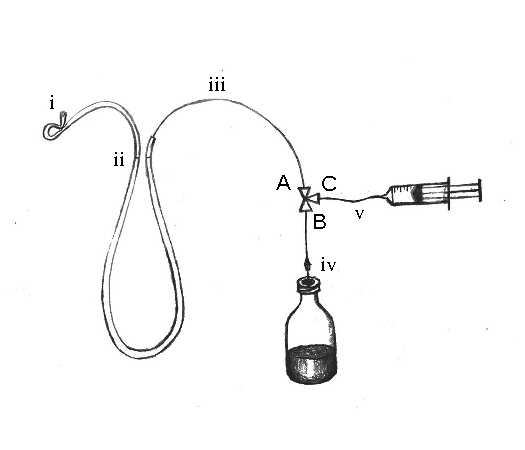
\includegraphics[]{figs/GD_utube.pdf}
  \caption{Aufbau aus U-Rohr-Manometer und 3-Wege-Ventil zur Messung des produzierten Biogases. Die gestrichelte Linie umgibt das einfache U-Rohr-Manometer, das durch ein digitales Manometer ersetzt werden kann. Detaillierte Erläuterungen zum Aufbau und Durchführung sind in Abschnitt \ref{sec:volmeas} zu finden.} 
  \label{fig:utube}
\end{figure}

\subsection{Schritt-für-Schritt-Anleitung Gasmessung}
\label{sec:steps}
\begin{enumerate}
    \item Messen und notieren Sie Raumtemperatur und  -druck, bei denen das Biogasvolumen bestimmt wird.
    \item Nehmen Sie die 3 Kontrollflaschen aus dem Inkubator und wiegen Sie sie, um die Konsistenz der Waage zu prüfen.
      Wenn die Ergebnisse mit den Anfangsmassen übereinstimmen bzw. innerhalb der erwarteten Genauigkeit liegen, fahren Sie fort. Falls nicht, identifizieren und beheben Sie das Problem mit der Waage oder ersetzen Sie die Waage, falls erforderlich.
      Wenn das Problem nicht gelöst werden kann, fahren Sie fort und korrigieren Sie später die Messergebnisse bezüglich der Skalendrift.\footnote{
        Die Korrektur erfolgt durch Berücksichtigung der durchschnittlichen scheinbaren Massendifferenz in den Kontrollflaschen bei allen Massenmessungen, die während dieser Gasmessung durchgeführt wurden.
        Wenn beispielsweise die Wasserkontrollen an Tag 4 durchschnittlich 0,1 g mehr wogen als zu Beginn, sollten die gemessenen Massen von \textit{allen} Flaschen am Tag 4 um 0,1 g nach unten korrigiert werden.
      }
    \item Entnehmen Sie einen Satz Replikate aus dem Inkubator (z.B. die drei Replikate für Cellulose).
    \item Es ist sinnvoll, immer mit demselben Replikat zu beginnen (z.B. \glqq 1\grqq{} oder \glqq a\grqq{}).\footnote{
        In diesem Fall kann die Auswirkung einer allmählichen Abkühlung des Kopfraums auf den Messfehler, der als gering einzuschätzen ist, quantifiziert werden, indem das BMP aus den einzelnen Replikaten über alle Substrate hinweg verglichen wird. Ein möglicher Einfluss würde sich derart bemerkbar machen, dass die ermittelte Gasproduktion mit steigender laufender Nummer (\glqq1, 2, 3, ...\grqq{} bzw. \glqq a, b, c, ...\grqq{}) statistisch signifikant über alle getesteten Substrate sinken würde.}
        Schwenken Sie die Flasche vorsichtig mindestens 10 Sekunden lang (aber nicht schütteln!), um den Inhalt zu mischen und ein Gleichgewicht zwischen dem \ce{CO2} in der Lösung und im Kopfraum sicherzustellen.
      Vermeiden Sie während des Schwenkens den Kontakt zwischen der Gärflüssig"=keit und dem Septum, um mögliche Massenverluste bei der Gasmessung zu vermeiden.\footnote{
        Wenn das Septum mit Gärflüssigkeit benetzt wird, kann aufgrund des herrschenden Überdruckes während der Gasmessung eine kleine Menge herausgedrückt werden, was zu Fehlern bei der Bestimmung des Massenverlusts führt. In Anbetracht des notwendigen, relativ großzügigen Kopfraumvolumens, kann in der Regel durch alleiniges Schwenken eine gute Durchmischung erreicht werden. Wenn das Septum dennoch mit Gärflüssigkeit in Kontakt kommt, notieren Sie sich das Auftreten und berücksichtigen Sie es später bei der Interpretation der Ergebnisse.
        Wenn der Verlust gering ist und es keinen merklichen Unterschied zwischen den Replikaten gibt, kann das Problem ignoriert werden; andernfalls sollten die Daten aus dem betroffenen Replikat verworfen werden.
      }
    \item Wiegen Sie die Flasche und notieren Sie das Ergebnis als Masse vor der Gasmessung.
    \item Entfernen Sie mit einer Spritze das überschüssige Biogas und ermitteln Sie dessen Volumen (vgl. Abschnitt \ref{sec:volmeas}). Verhindern Sie, dass die Kanüle mit der Gärflüssigkeit in Kontakt kommt, indem Sie diese stets in der Gasphase halten.
      Verwenden Sie das Manometer, um sicherzustellen, dass sowohl der Druck des Biogases in der Spritze als auch der des Biogases in der Flasche, in etwa dem atmosphärischen Druck entspricht (Manometerdruck = 0 $\pm$ 3 kPa).
    \item Wiegen Sie die Flasche nach der Gasmessung und notieren Sie das Ergebnis als Masse nach der Gasmessung.
    \item Fahren Sie mit dem nächsten Replikat fort (z.B. \glqq 2\grqq{} oder \glqq b\grqq{}) und wiederholen Sie die Schritte 4 bis 7.
    \item Nachdem alle Replikate homogenisiert, gewogen, entgast und erneut gewogen wurden, stellen Sie die Flaschen wieder in den Inkubator.
    Fahren Sie mit dem nächsten Satz an Replikaten fort (z.B. den drei Wiederholungen für das Substrat \glqq Bioabfall A\grqq{}) und wiederholen Sie die Schritte 3 bis 9.
\end{enumerate}

Diese Abfolge der einzelnen Schritte ist schematisch in Abb. \ref{fig:steps} dargestellt.\footnote{
    Wenn das System von mehreren ggf. noch wenig erfahrenen Anwendern genutzt wird, kann es sinnvoll sein, Abb. \ref{fig:steps} auszudrucken und in der Nähe der Waage auszulegen, damit die Vorgehensweise bei den routinemäßigen Gasmessungen verinnerlicht wird.}

\begin{figure}[ht]
  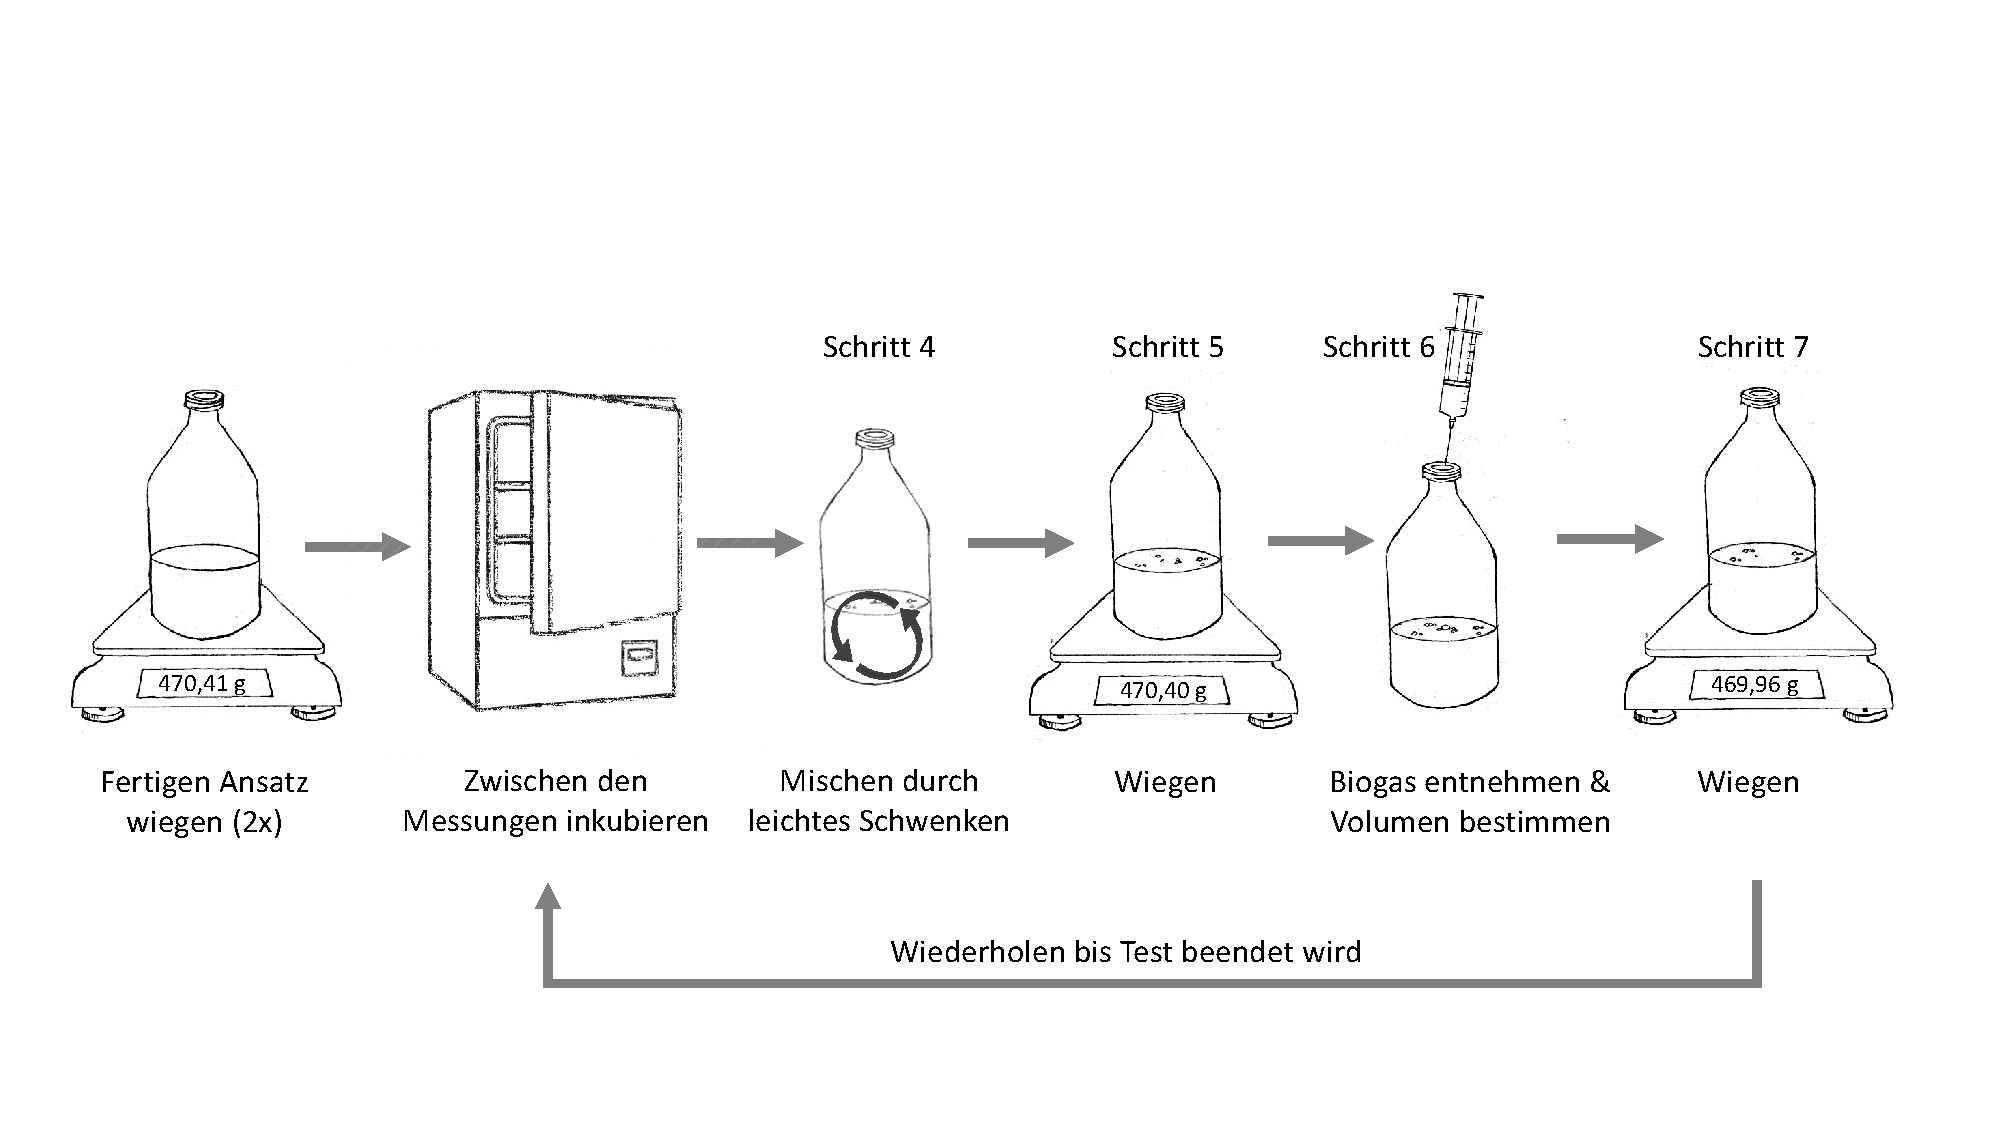
\includegraphics[width=\textwidth]{figs/GD_steps_DE.pdf}
  \caption{Die erforderlichen Schritte bei der Gasmessung in der GD-BMP-Methode. Die Nummern der Schritte entsprechen den im Text aufgeführten und werden bei jeder Gasmessung wiederholt. Für Einzelheiten zur Volumenmessung (Schritt 6) siehe Abschnitt \ref{sec:volmeas}.}
  \label{fig:steps}
\end{figure}


\section{Qualitätskontrolle}
Die GD-BMP-Methode erfordert eine genaue Bestimmung des Gasvolumens und des Massenverlusts der Flaschen.
Es ist wichtig, dass jedes neue Setup getestet wird; sinnvollerweise sollte die Prüfung regelmäßig oder zumindest nach vorgenommenen Veränderungen erfolgen.
Glücklicherweise kann einfach Umgebungsluft als Standard verwendet werden.
Um die Funktionalität des Systems zu testen, verwenden Sie einfach eine Spritze, um \textit{vorsichtig} ein Volumen (erfahrungemäß geht nicht viel mehr als etwa 20 \%) in eine leere (aber mit Umgebungsluft auf Umgebungsdruck gefüllte) Flasche zu pressen, und fahren Sie mit den oben angegebenen Messschritten fort.
Berechnen Sie die Dichte von Luft basierend auf dem Massenverlust der Flasche durch das Entgasen auf Umgebungsdruck und dem Volumen des entfernten Gases.\footnote{Dieses Volumen ist normalerweise aufgrund von minimalen Undichtigkeiten beim Anschließen und/oder Entfernen der Spritze etwas kleiner als das anfänglich hinzugefügte Volumen.}
Der Wert sollte innerhalb von 10 \% (oder besser 5 \%) der Dichte für den vorliegenden Umgebungsdruck und die Raumtemperatur liegen.\footnote{Die Luftdichte kann z.B. unter folgendem Link berechnet werden:  \url{https://www.density.co.uk/calculators/density-of-air/}. Der Einfluss der Luffeuchte ist bei Raumtemperatur gering (unter der Annahme einer Temperatur $\le$ 25$^\circ$C). Die Dichte beträgt 1,20 mg ml$^{-1}$ für trockene Luft bei 20 $^\circ$ C und 101,3 kPa und 1,19 mg ml$^{-1}$, wenn sie mit Wasser gesättigt ist.}

\section{Berechnungen}
In Dokument 204 der Website für Standard-BMP-Methoden \citep{BMPdoc204gasdens} finden Sie eine detaillierte Beschreibung der Berechnungen für die GD-BMP-Methode.
Berechnungen können auch mit der kostenlosen Web-App OBA (\url{https://biotransformers.shinyapps.io/oba1/}) oder dem Biogaspaket in R (\url{https://cran.r-project.org/package=biogas}) \citep{hafnerSoftwareBiogasResearch2018} durchgeführt werden.
Die finalen Ergebnisse sollten immer basierend auf den derzeit gültigen Validierungskriterien bewertet werden \citep{BMPdoc100req}.

\bibliography{bib}

\end{document}


